\documentclass[sigplan,screen]{acmart}

\usepackage{booktabs} % For formal tables
\usepackage{cleveref}
\usepackage{hyperref}
\usepackage{natbib}
\usepackage[utf8]{inputenc}


% Copyright
\setcopyright{rightsretained}
\acmDOI{}
\acmISBN{}
\acmConference[PriSC]{Workshop on Principles of Secure Compilation}{2018}{Los Angeles} 
\acmYear{2018}
\copyrightyear{2018}
\settopmatter{printacmref=false}

% \acmPrice{15.00}

%\acmBadgeL[http://ctuning.org/ae/ppopp2016.html]{ae-logo}
%\acmBadgeR[http://ctuning.org/ae/ppopp2016.html]{ae-logo}


\begin{document}
\title{Enforcing Well-bracketed Control Flow and Stack Encapsulation using Linear Capabilities}
% \titlenote{Produces the permission block, and
%   copyright information}
\subtitle{Extended Abstract}
% \subtitlenote{The full version of the author's guide is available as
%   \texttt{acDat zou in dmart.pdf} document}

\author{Lau Skorstengaard}
% \orcid{}
\affiliation{%
  \institution{Aarhus University}
}
\email{lau@cs.au.dk}

\author{Dominique Devriese}
\orcid{0000-0002-3862-6856}
\affiliation{%
  \institution{imec-DistriNet, KU Leuven}
}
\email{dominique.devriese@cs.kuleuven.be}

\author{Lars Birkedal}
\affiliation{%
  \institution{Aarhus University}
}
\email{birkedal@cs.au.dk}

% The default list of authors is too long for headers}
% \renewcommand{\shortauthors}{B. Trovato et al.}

\begin{abstract}
We propose and study a new calling convention that provably enforces well-bracketed control flow and local state encapsulation on a capability machine.
The calling convention is based on linear capabilities, a type of capabilities that are prevented by the hardware from being duplicated.
In addition to designing and formalising this new calling convention, we also contribute a new way to formalise and prove that it effectively enforces well-bracketed control flow and local state encapsulation, building on the concept of fully abstract compilation.
\end{abstract}

%
% The code below should be generated by the tool at
% http://dl.acm.org/ccs.cfm
% Please copy and paste the code instead of the example below. 
%
% \begin{CCSXML}
% <ccs2012>
%  <concept>
%   <concept_id>10010520.10010553.10010562</concept_id>
%   <concept_desc>Computer systems organization~Embedded systems</concept_desc>
%   <concept_significance>500</concept_significance>
%  </concept>
%  <concept>
%   <concept_id>10010520.10010575.10010755</concept_id>
%   <concept_desc>Computer systems organization~Redundancy</concept_desc>
%   <concept_significance>300</concept_significance>
%  </concept>
%  <concept>
%   <concept_id>10010520.10010553.10010554</concept_id>
%   <concept_desc>Computer systems organization~Robotics</concept_desc>
%   <concept_significance>100</concept_significance>
%  </concept>
%  <concept>
%   <concept_id>10003033.10003083.10003095</concept_id>
%   <concept_desc>Networks~Network reliability</concept_desc>
%   <concept_significance>100</concept_significance>
%  </concept>
% </ccs2012>  
% \end{CCSXML}

% \ccsdesc[500]{Computer systems organization~Embedded systems}
% \ccsdesc[300]{Computer systems organization~Redundancy}
% \ccsdesc{Computer systems organization~Robotics}
% \ccsdesc[100]{Networks~Network reliability}


% \keywords{ACM proceedings, \LaTeX, text tagging}

% \begin{teaserfigure}
%   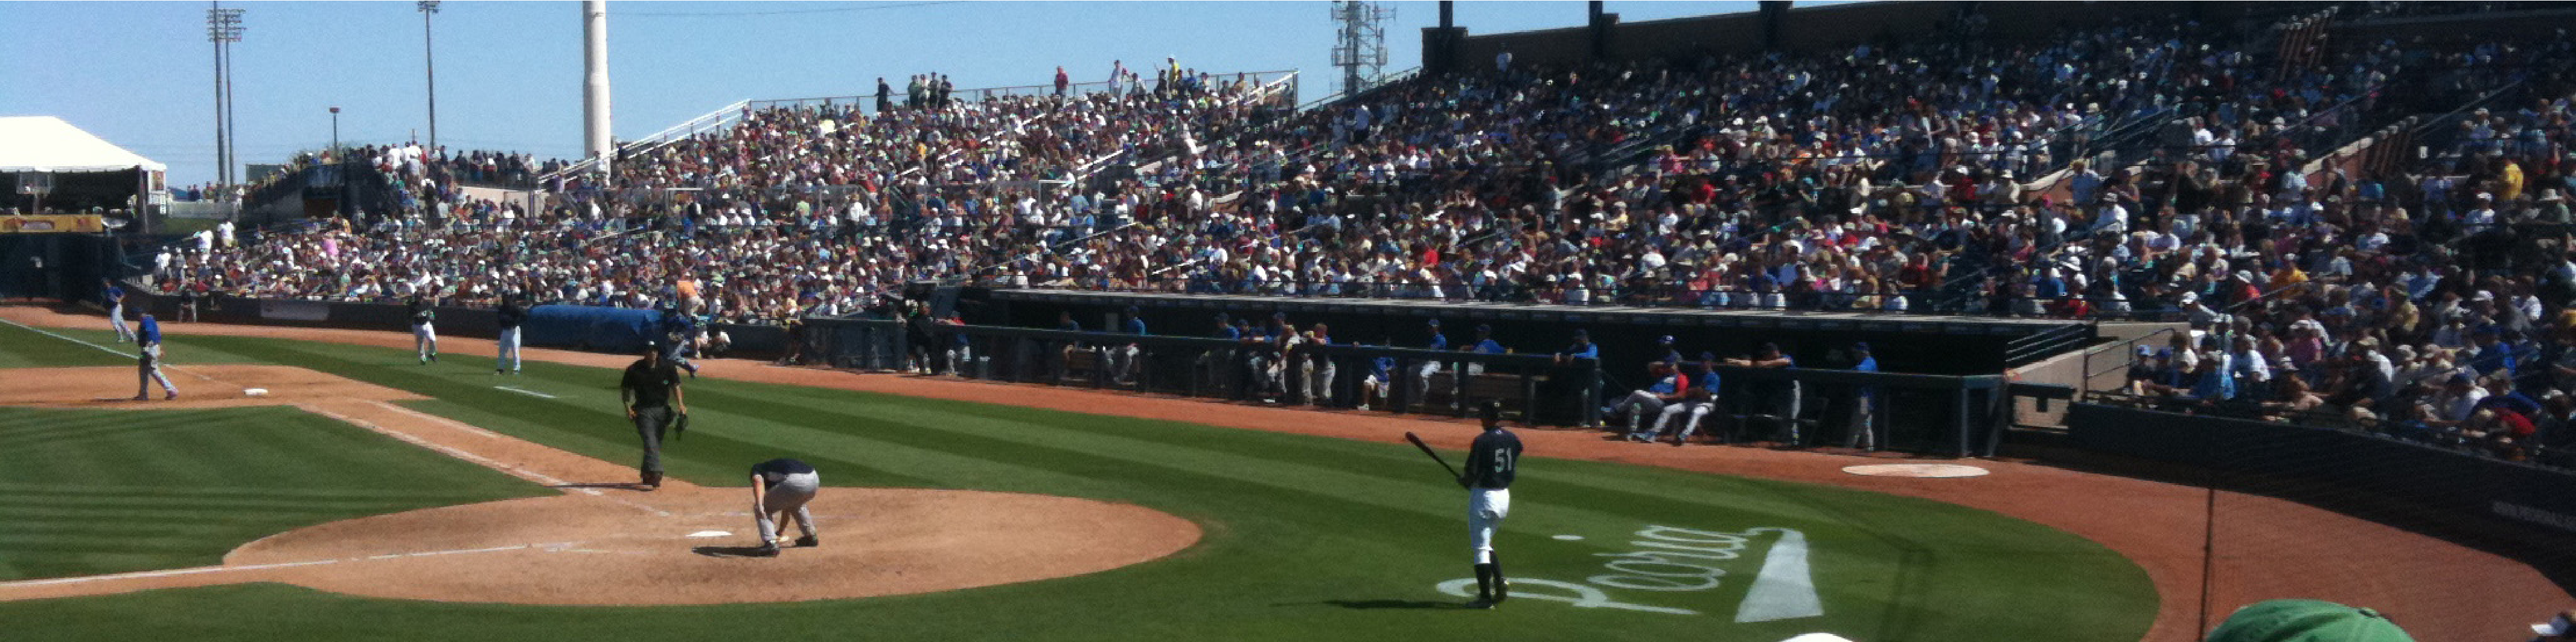
\includegraphics[width=\textwidth]{sampleteaser}
%   \caption{This is a teaser}
%   \label{fig:teaser}
% \end{teaserfigure}


\maketitle

\section{Introduction}
Secure compilers preserve source-language (security-relevant) properties even when the compiled code interacts with arbitrary target-language components.
Generally, properties that hold in the source language but not in the target language, need to be somehow enforced by the compiler.
Two properties that hold in many high-level source languages, but not in the assembly languages they are compiled to, are well-bracketed control flow and encapsulation of local state.

Well-bracketed control flow expresses that invoked functions must either return to their callers, invoke other functions themselves or diverge, and generally holds in programming languages that do not offer a primitive form of continuations. 
At the assembly level, this is not so obvious, as invoked functions get direct access to return pointers, that they are supposed to jump to a single time, at the end of their execution, but there is no guarantee that untrusted assembly code respects this intended usage.
Particularly, a function may invoke return pointers from other stack frames than its own: either frames higher in the call stack or ones that no longer exist as they have already returned before. 

Local state encapsulation is the guarantee that when a function invokes another function, its local variables will not have been modified when the invoked function returns.
At the assembly level, this property is also far from obvious.
The calling function's local variables are stored on the stack during the invocation, and functions are not supposed to touch stack frames other than their own.
However, untrusted assembly code is free to ignore this requirement and overwrite the local state of its caller or other stack frames.

To enforce these properties, target language security primitives are needed that can be used to prevent untrusted code from misbehaving, without imposing too much overhead on well-behaved code.
The virtual-memory based security primitives on commodity processors do not seem sufficiently fine-grained to efficiently support this.
More suitable security primitives are offered by a type of processors known as capability machines \citep{levy_capability-based_1984,watson_cheri:_2015}.
These processors use tagged memory to enforce a strict separation between integers and \emph{capabilities}: pointers that carry authority.
Capabilities come in different flavours.
Memory capabilities are used to read from and write to memory.
Additionally, the CHERI capability machine offers sealed code-data pairs of capabilities that represent an encapsulated closure: a piece of code coupled with private state that it gains access to upon invocation.\footnote{Other capability machines offer other mechanisms that can be used to the same effect.} 

CheriBSD, an operating system built on CHERI, uses per-component separate stacks and a central, trusted stack manager component to enforce well-bracketed control flow and private state encapsulation \citep{watson_cheri:_2015}.
To prevent the stack pointer (or derivatives) from being passed to other components, CheriBSD uses local capabilities: a type of capabilities that can be kept in registers but not stored in memory (except through store-local capabilities like the stack pointer itself).
The literature does not contain many details about the mechanism, let alone a formal analysis, but additionally, the mechanism does not seem able to support higher-order interfaces (e.g. C function pointers) in a scalable fashion.

In recent work, we have been looking at an alternative approach \citep{skorstengaard_reasoning_2017}.
We also use CHERI's local capabilities, but combine them with a more traditional, single, shared stack that scales better in the presence of higher-order interfaces.
By passing stack and return pointers as local capabilities, we effectively prevent callees from storing them on the heap.
Using a step-indexed Kripke logical relation, we are able to prove correctness of programs that rely on well-bracketed control flow in a complex way.

While this approach works quite well, this paper investigates another alternative approach.
We aim to make two improvements, discussed in the next sections: (1) remove the need to clear the stack on boundary crossings and (2) explore a new formal statement of well-bracketed control flow and local state encapsulation.

\section{Linear Capabilities, not Local}
What we essentially want to achieve in a secure calling convention is to give an invoked function access to a stack pointer and a return pointer, but only temporarily: during the execution of the invoked function. 
In our original approach, we make both pointers local, so that the CHERI processor guarantees, essentially, that they can only be stored in registers or on the stack.
To prevent an invoked function from transferring the pointers across outside the lifetime of its stack frame, it then suffices to block only these two communication channels, rather than the entire memory.
In other words, we need to clear registers and the stack before passing control to untrusted code, to prevent it from obtaining access to stack and return pointers for other stack frames than its own.
The requirement for clearing registers is unproblematic, but clearing the entire stack upon every boundary crossing is a non-trivial requirement.
We speculate that it can be made efficient with custom hardware extensions\footnote{Specifically, we imagine a kind of pre-L0 processor cache that does not retain values but only remembers that a certain range has been zeroed out.}, but this is not obvious.

An alternative that does not have this requirement, relies on \emph{linear capabilities}, rather than local ones.
Although details in the literature are scarce, linear capabilities have already been implemented in the SAFE machine~\citep{amorim_verified_2014}\footnote{Private communication with Catalin Hrit\c{c}u.} and considered for implementation in CHERI\footnote{Private communication with Robert Watson.}.
The idea is that all capabilities are marked as either regular or linear.
Linear ones are subject to special hardware-enforced restrictions, that prevent them from being duplicated.
For example, when linear capabilities are moved to a new location in registers or memory, they are erased from their old location.
A few special instructions are needed to make this workable, e.g.\ a split instruction that splits a memory capability for a region of memory into disjoint capabilities for two parts of the region and a splice instruction that does the reverse.
This linearity is a powerful tool: when passing a linear capability to untrusted code and receiving the same capability back, we are sure that they cannot have stored a copy of it.
Similarly, when we receive, from untrusted code, a linear capability that addresses memory that we know is only ever addressed by linear capabilities, then we are sure that the untrusted code no longer has access that memory.

As such, linear capabilities can be used as an alternative to local capabilities to enforce well-bracketed control flow.
We cannot provide full details here for space reasons, but the idea is essentially the following.
By passing stack and return pointers as linear capabilities, and requiring that invoked functions hand in their stack pointer upon return, untrusted code is prevented from holding on to stack and return pointers past their intended lifetime, essentially because they can only ever have one copy and they have to hand it in when this lifetime ends.

\section{Formalising well-bracketed control flow}
The second improvement we are making is related to the properties of well-bracketed control flow and local state encapsulation.
To establish these properties, our previous work followed previous work \citep{dreyer_impact_2010} in providing a sound reasoning technique and using it to prove soundness of challenging example programs that rely on the properties.
In the current work, we are investigating an alternative way to formalise the two properties, based on the notion of fully abstract compilation \citep{abadi_protection_1999}.

We intend to start by formalising the assembly language for a capability machine with linear capabilities (the target language).
Then, we will introduce the source language: a variant of this target language that features a primitive stack, built into the operational semantics, as well as additional instructions like call.
While the target language is a standard assembly language without even the notion of a stack, the source language does have a stack, and control flow well-bracketedness and local state encapsulation follow more directly from the operational semantics.
We will formalise our calling convention in the definition of a compiler from the source to the target language.
Additionally, we conjecture that this compiler can be proved fully abstract, thus formally expressing and establishing security of the calling convention.

Interestingly, the proof of full abstraction for this compiler is expected to use a very simple back-translation, that simply maps every target language instruction to the corresponding instruction in the source.
This back-translation works because we construct our source language in such a way that it has direct counterparts to every target language value.
Specifically, the source language contains a representation of stack and return pointers as unspecified abstract values whose behavior corresponds to their target counterparts, but in a way that guarantees the intended properties of well-bracketed control flow and local state encapsulation.

\bibliographystyle{ACM-Reference-Format}
\bibliography{references} 

\end{document}
